\chapter{Vulnerability assessment}
 Vulnerability Assessment aims to identify and categorize risks for security
 weaknesses related to assets within an environment. It is important to note
 that there is little to no manual exploitation during a vulnerability
 assessment. A vulnerability assessment also provides remediation steps to fix
 the issues.

The purpose of a Vulnerability Assessment is to understand, identify, and
categorize the risk for the more apparent issues present in an environment
without actually exploiting them to gain further access. Depending on the scope
of the assessment, some customers may ask us to validate as many
vulnerabilities as possible by performing minimally invasive exploitation to
confirm the scanner findings and rule out false positives. Other customers will
ask for a report of all findings identified by the scanner. As with any
assessment, it is essential to clarify the scope and intent of the
Vulnerability Assessment before starting. Vulnerability management is vital to
help organizations identify the weak points in their assets, understand the
risk level, and calculate and prioritize remediation efforts.

It is also important to note that organizations should always test substantial
patches before pushing them out into their environment to prevent disruptions.

\section{Methodology}

Below is a sample Vulnerability Assessment methodology that most organizations
could follow and find success with. Methodologies may vary slightly from
organization to organization, but this chart covers the main steps, from
identifying assets to creating a remediation plan. 


\begin{figure}
  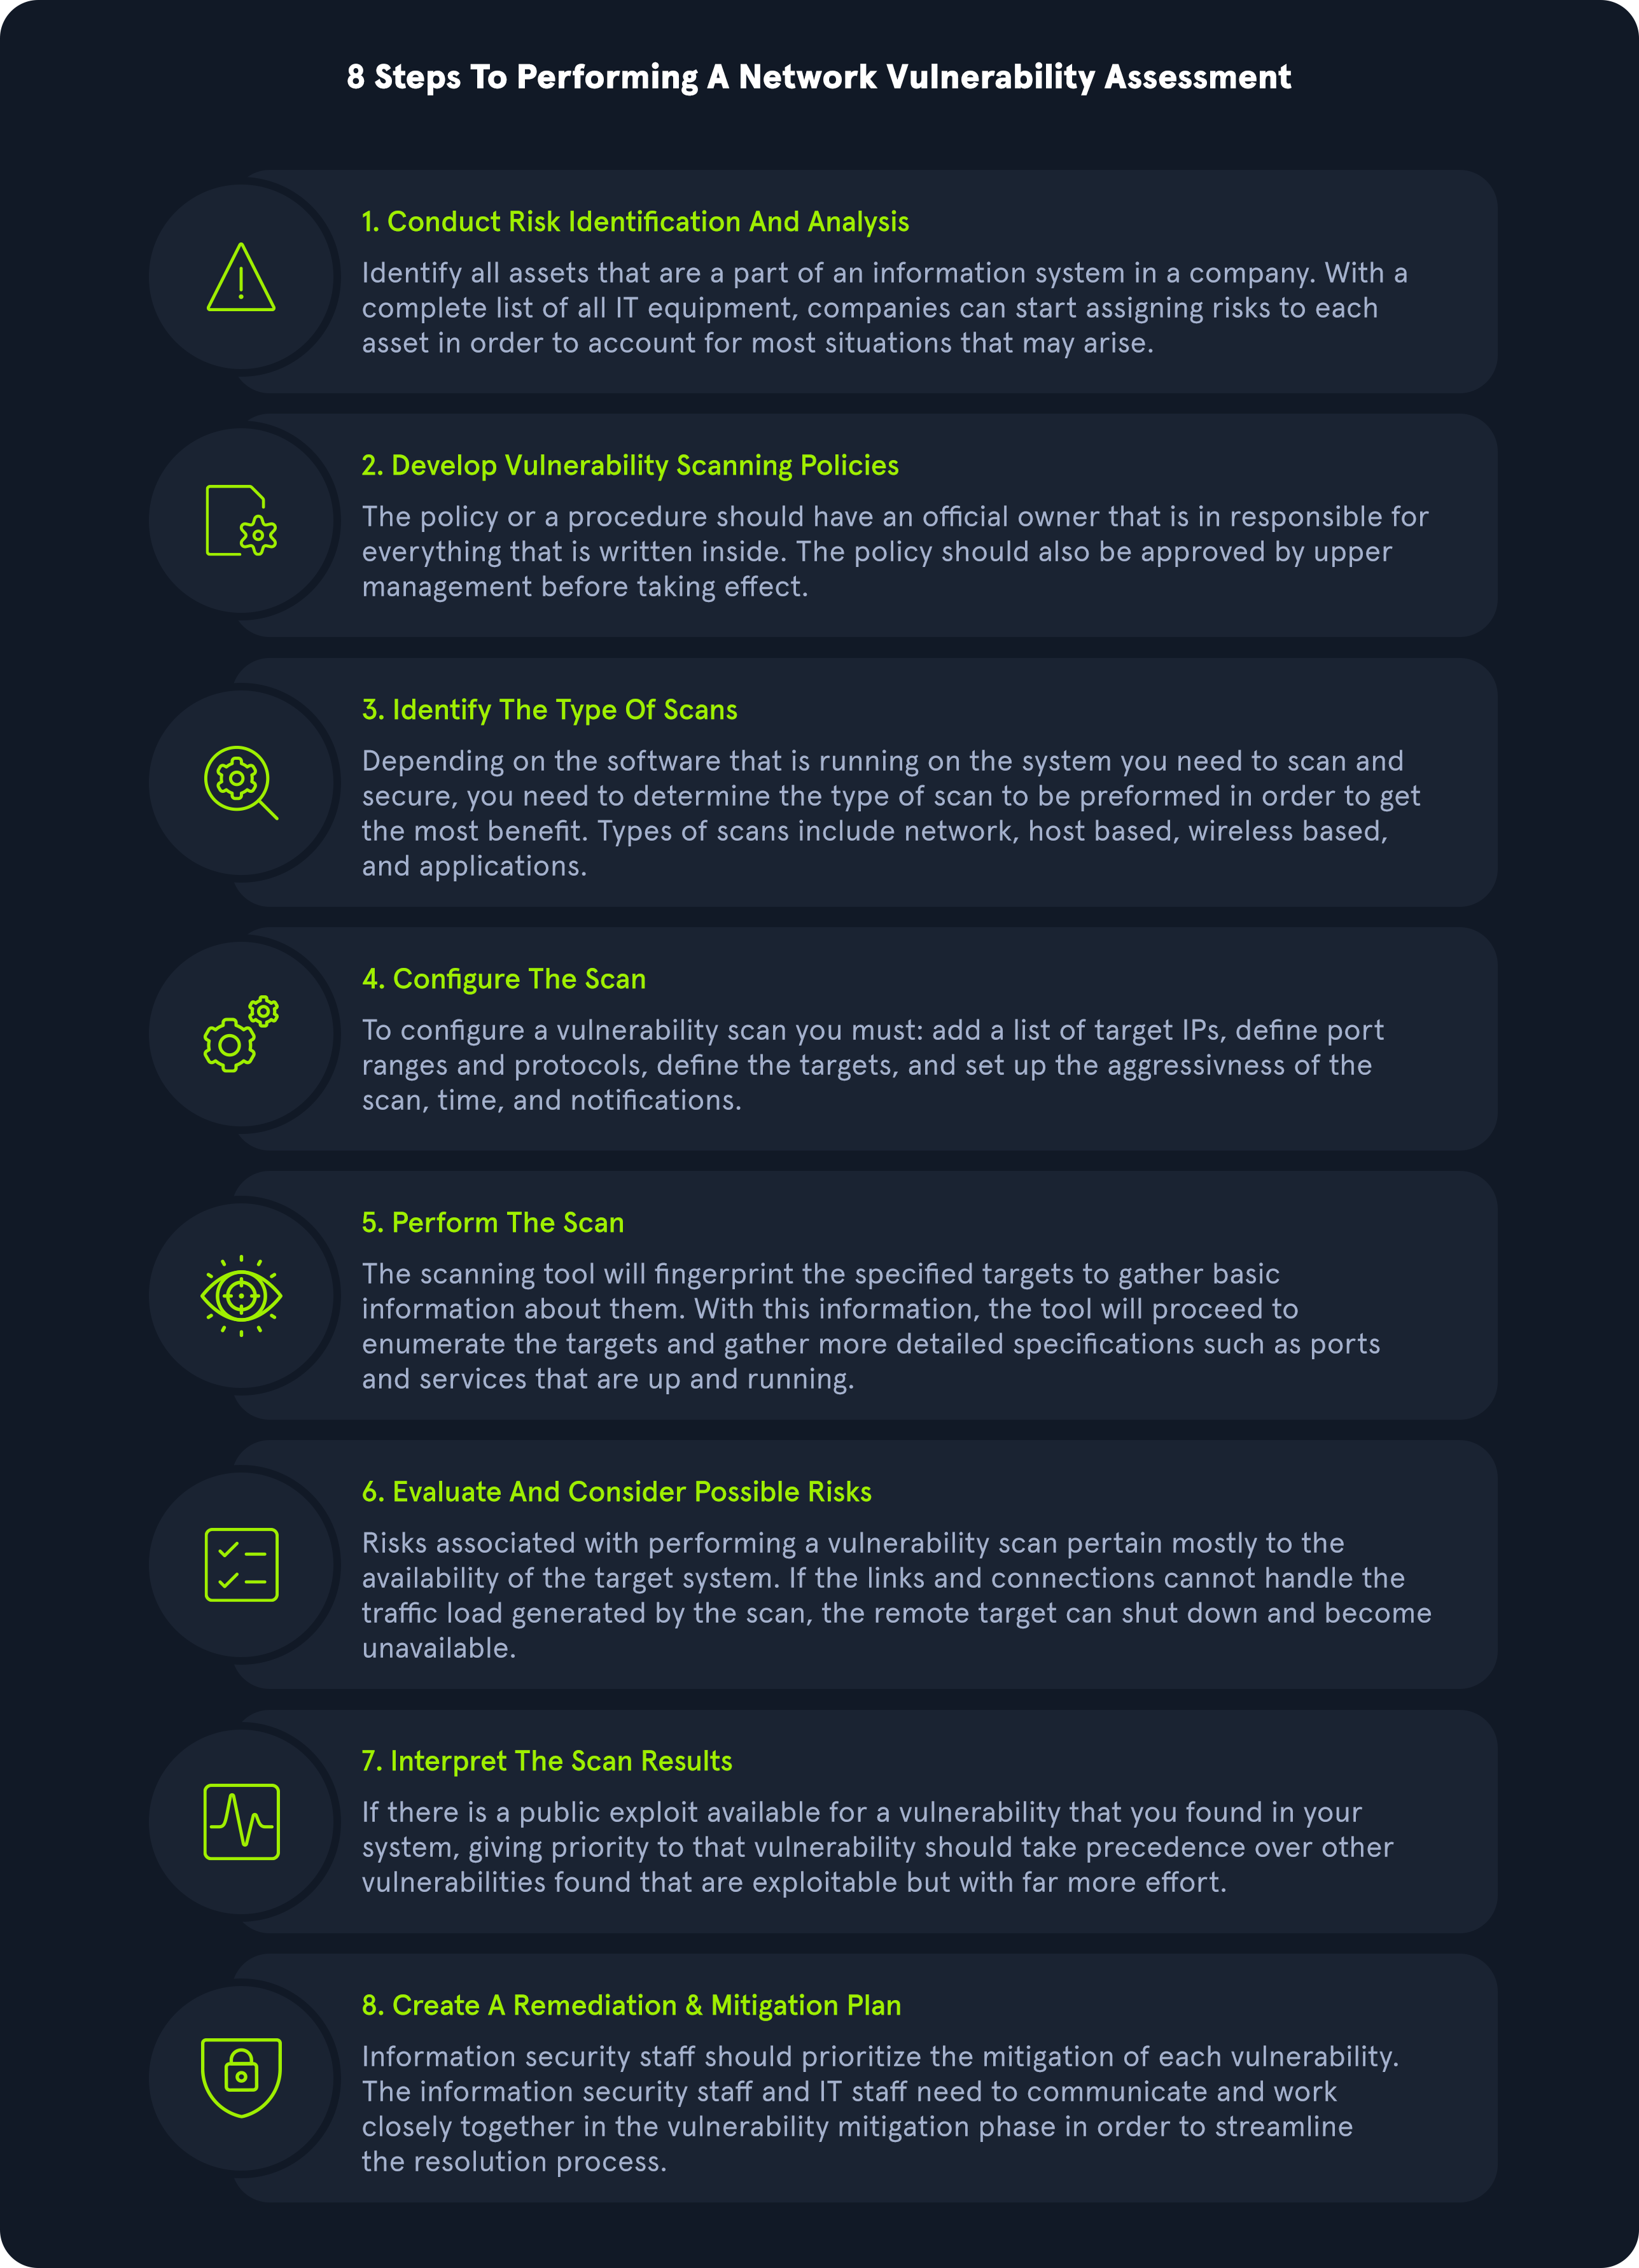
\includegraphics[width=\linewidth]{intro/vuln/images/methodo.png}
  \caption{Methodology}
  \label{fig:pentest-vul-methodo}
\end{figure}

\section{Key Terms}
{\bf Vulnerability}

A Vulnerability is a weakness or bug in an organization's environment,
including applications, networks, and infrastructure, that opens up the
possibility of threats from external actors. Vulnerabilities can be registered
through MITRE's Common Vulnerability Exposure database and receive a Common
Vulnerability Scoring System (CVSS) score to determine severity. This scoring
system is frequently used as a standard for companies and governments looking
to calculate accurate and consistent severity scores for their systems'
vulnerabilities. Scoring vulnerabilities in this way helps prioritize resources
and determine how to respond to a given threat. Scores are calculated using
metrics such as the type of attack vector (network, adjacent, local, physical),
the attack complexity, privileges required, whether or not the attack requires
user interaction, and the impact of successful exploitation on an
organization's confidentiality, integrity, and availability of data. Scores can
range from 0 to 10, depending on these metrics.

{\bf Threat}

A Threat is a process that amplifies the potential of an adverse event, such as
a threat actor exploiting a vulnerability. Some vulnerabilities raise more
threat concerns over others due to the probability of the vulnerability being
exploited. For example, the higher the reward of the outcome and ease of
exploitation, the more likely the issue would be exploited by threat actors.

{\bf Exploit}

An Exploit is any code or resources that can be used to take advantage of an asset's weakness. Many exploits are available through open-source platforms such as Exploitdb or the Rapid7 Vulnerability and Exploit Database. We will often see exploit code hosted on sites such as GitHub and GitLab as well.

{\bf Risk}

Risk is the possibility of assets or data being harmed or destroyed by threat actors.

To differentiate the three, we can think of it as follows:
\begin{itemize}
        \item Risk: something bad that could happen
        \item Threat: something bad that is happening
        \item Vulnerabilities: weaknesses that could lead to a threat
\end{itemize}

Vulnerabilities, Threats, and Exploits all play a part in measuring the level
of risk in weaknesses by determining the likelihood and impact. For example,
vulnerabilities that have reliable exploit code and are likely to be used to
gain access to an organization's network would significantly raise the risk of
an issue due to the impact. If an attacker had access to the internal network,
they could potentially view, edit, or delete sensitive documents crucial for
business operations. We can use a qualitative risk matrix to measure risk based
on likelihood.


\section{Common Vulnerability Scoring System (CVSS)}

There are various ways to score or calculate severity ratings of
vulnerabilities. The Common Vulnerability Scoring System (CVSS) is an industry
standard for performing these calculations. Many scanning tools will apply
these scores to each finding as a part of the scan results, but it's important
that we understand how these scores are derived in case we ever need to
calculate one by hand or justify the score applied to a given vulnerability.
Risk Scoring

The CVSS system helps categorize the risk associated with an issue and allows
organizations to prioritize issues based on the rating. The CVSS scoring
consists of the exploitability and impact of an issue. The exploitability
measurements consist of access vector, access complexity, and authentication.
The impact metrics consist of the CIA triad, including confidentiality,
integrity, and availability.

\begin{figure}
  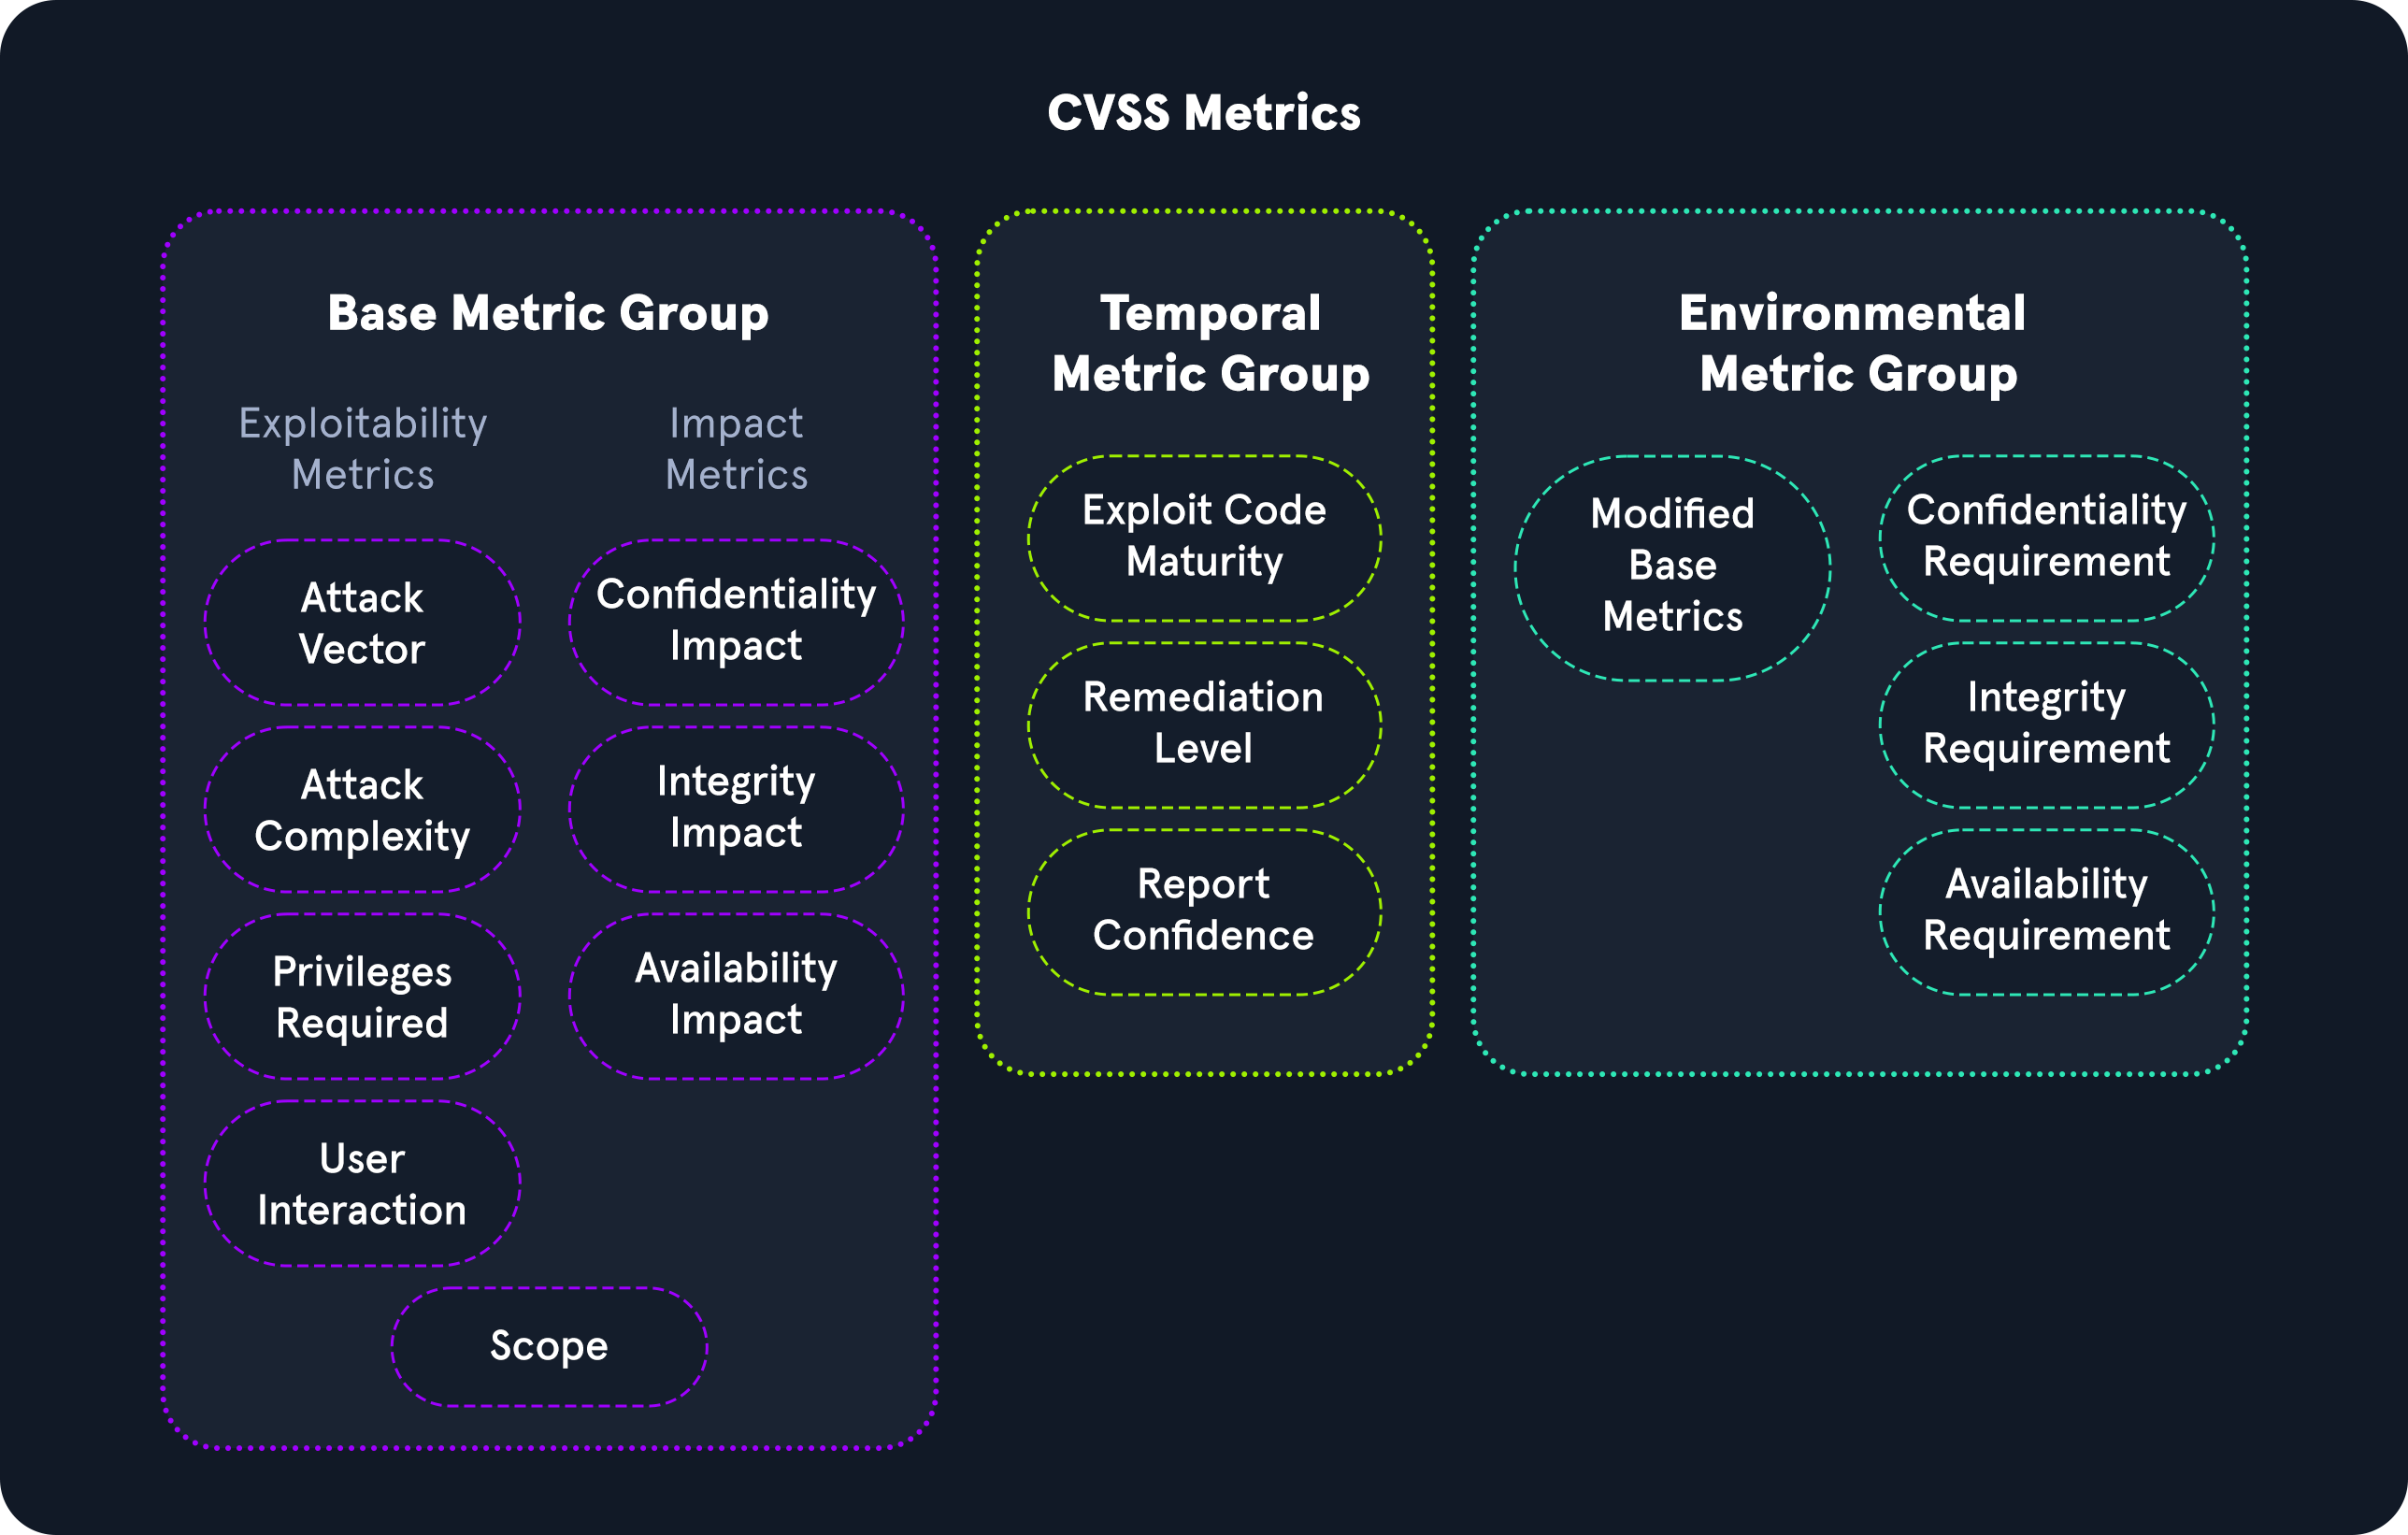
\includegraphics[width=\linewidth]{intro/vuln/images/cvss.png}
  \caption{CVSS}
  \label{fig:pentest-vul-cvss}
\end{figure}
\subsection{Base Metric Group}

The CVSS base metric group represents the vulnerability characteristics and consists of exploitability metrics and impact metrics.

\subsubsection{Exploitability Metrics}

The Exploitability metrics are a way to evaluate the technical means needed to exploit the issue using the metrics below:
\begin{itemize}
    \item Attack Vector
    \item Attack Complexity
    \item Privileges Required
    \item User Interaction
\end{itemize}

\subsubsection{Impact Metrics}

The Impact metrics represent the repercussions of successfully exploiting an issue and what is impacted in an environment, and it is based on the CIA triad. The CIA triad is an acronym for Confidentiality, Integrity, and Availability.

\subsection{Temporal Metric Group}

The Temporal Metric Group details the availability of exploits or patches regarding the issue.

\subsubsection{Exploit Code Maturity}

The Exploit Code Maturity metric represents the probability of an issue being exploited based on ease of exploitation techniques. There are various metric values associated with this metric, including Not Defined, High, Functional, Proof-of-Concept, and Unproven.

A 'Not Defined' value relates to skipping this particular metric. A 'High' value represents an exploit consistently working for the issue and is easily identifiable with automated tools. A Functional value indicates there is exploit code available to the public. A Proof-of-Concept demonstrates that a PoC exploit code is available but would require changes for an attacker to exploit the issue successfully.

\subsubsection{Remediation Level}

The Remediation level is used to identify the prioritization of a vulnerability. The metric values associated with this metric include Not Defined, Unavailable, Workaround, Temporary Fix, and Official Fix.

A 'Not Defined' value relates to skipping this particular metric. An 'Unavailable' value indicates there is no patch available for the vulnerability. A 'Workaround' value indicates an unofficial solution released until an official patch by the vendor. A 'Temporary Fix' means an official vendor has provided a temporary solution but has not released a patch yet for the issue. An 'Official Fix' indicates a vendor has released an official patch for the issue for the public.

\subsubsection{Report Confidence}

Report Confidence represents the validation of the vulnerability and how accurate the technical details of the issue are. The metric values associated with this metric include Not Defined, Confirmed, Reasonable, and Unknown.

A 'Not Defined' value relates to skipping this particular metric. A 'Confirmed' value indicates there are various sources with detailed information confirming the vulnerability. A 'Reasonable' value indicates sources have published information about the vulnerability. However, there is no complete confidence that someone would achieve the same result due to missing details of reproducing the exploit for the issue.

\subsection{Environmental Metric Group}

The Environmental metric group represents the significance of the vulnerability of an organization, taking into account the CIA triad.

\subsubsection{Modified Base Metrics}

The Modified Base metrics represent the metrics that can be altered if the affected organization deems a more significant risk in Confidentiality, Integrity, and Availability to their organization. The values associated with this metric are Not Defined, High, Medium, and Low.

A 'Not Defined' value would indicate skipping this metric. A 'High' value would mean one of the elements of the CIA triad would have astronomical effects on the overall organization and customers. A 'Medium' value would indicate one of the elements of the CIA triad would have significant effects on the overall organization and customers. A 'Low' value would mean one of the elements of the CIA triad would have minimal effects on the overall organization and customers.

\subsection{Calculating CVSS Severity}

The calculation of a CVSS v3.1 score takes into account all the metrics
discussed in this section. The National Vulnerability Database has a calculator
available to the public
\href{https://nvd.nist.gov/vuln-metrics/cvss/v3-calculator}{here}.


\section{Open Vulnerability Assessment Language (OVAL)}
\href{https://oval.mitre.org/}{Open Vulnerability Assessment Language} (OVAL)
is a publicly available information security international standard used to
evaluate and detail the system's current state and issues. OVAL is also
co-supported by the office of Cybersecurity and Communications from the U.S.
Department of Homeland Security. OVAL provides a language to understand
encoding system attributes and various content repositories shared within the
security community. The OVAL repository has over 7000+ definitions for public
use. Additionally, OVAL is also used by the U.S. National Institute of
Standards and Technology's (NIST) Security Content Automation Protocol (SCAP)
which brings together community ideas for automating vulnerability management,
measurement, and ensuring systems meet policy compliance.

The goal of the OVAL language is to have a three-step structure during the
assessment process that consists of:
\begin{itemize}
        \item Identifying a system's configurations for testing
        \item Evaluating the current system's state
        \item Disclosing the information in a report
\end{itemize}

The information can be described in various types of states, including: Vulnerable, Non-compliant, Installed Asset, and Patched.

The OVAL definitions are recorded in an XML format to discover any software vulnerabilities, misconfigurations, programs, and additional system information taking out the need to exploit a system. By having the ability to identify issues without directly exploiting the issue, an organization can correlate which systems need to be patched in a network.

The four main classes of OVAL definitions consist of:
\begin{itemize}
    \item  OVAL Vulnerability Definitions: Identifies system vulnerabilities
    \item  OVAL Compliance Definitions: Identifies if current system configurations meet system policy requirements
    \item  OVAL Inventory Definitions: Evaluates a system to see if a specific software is present
    \item  OVAL Patch Definitions: Identifies if a system has the appropriate patch
\end{itemize}

Additionally, the OVAL ID Format consist of a unique format that consists of
"oval:Organization Domain Name:ID Type:ID Value". The ID Type can fall into
various categories including: definition (def), object (obj), state (ste), and
variable (var). An example of a unique identifier would be 
\verb+oval:org.mitre.oval:obj:1116+.

Scanners such as Nessus have the ability to use OVAL to configure security
compliance scanning templates.

\section{Common Vulnerabilities and Exposures (CVE)}
\href{https://cve.mitre.org/}{Common Vulnerabilities and Exposures} (CVE) is a
publicly available catalog of security issues sponsored by the United States
Department of Homeland Security (DHS). Each security issue has a unique CVE ID
number assigned by the CVE Numbering Authority (CNA). The purpose of creating a
unique CVE ID number is to create a standardization for a vulnerability or
exposure as a researcher identifies it. A CVE consists of critical information
regarding a vulnerability or exposure, including a description and references
about the issue. The information in a CVE allows an organization's IT team to
understand how detrimental a problem could be to their environment.

ny vulnerabilities assigned a CVE must be:
\begin{itemize}
        \item independently fixable: the flaw can be fixed independently of any
            other bugs.
        \item affect just one codebase: flaws that impact more than one product
            get separete CVEs
        \item acknowledged and documented by the relevant vendor: the vendor
            acknowledges the bug and its negative impact on security Or the bug
            AND the violation of the security policy of the affected system
            must be documented.
\end{itemize}
\subsection{Responsible Disclosure}

Security researchers and consultants constantly reference the CVE database since it consists of thousands of vulnerabilities that could be leveraged for exploitation. In addition, there are also times when individuals may come across an issue they have never seen in the wild or it has never disclosed while digging into a specific software or program.

Responsible disclosure is essential in the security community because it allows an organization or researcher to work directly with a vendor providing them with the issue details first to ensure a patch is available before the vulnerability announcement to the world. If an issue is not responsibly disclosed to a vendor, real threat actors may be able to leverage the issues for criminal use, also referred to as a zero day or an 0-day.

\section{Vulnerability Scanning Overview}
As discussed earlier, vulnerability scanning is performed to identify potential
vulnerabilities in network devices such as routers, firewalls, switches, as
well as servers, workstations, and applications. Scanning is automated and
focuses on finding potential/known vulnerabilities on the network or at the
application level. Vulnerabilities scanners typically do not exploit
vulnerabilities (with some exceptions) but need a human to manually validate
scan issues to determine whether or not a particular scan returned real issues
that need to be fixed or false positives that can be ignored and excluded from
future scans against the same target.

Vulnerability scanning is often part of a standard penetration test, but the
two are not the same. A vulnerability scan can help gain additional coverage
during a penetration test or speed up the project's testing under time
constraints. An actual penetration test includes much more than just a scan.

The type of scans run varies from one tool to another, but most tools run a
combination of dynamic and static tests, depending on the target and the
vulnerability. A static test would determine a vulnerability if the identified
version of a particular asset has a public CVE. However, this is not always
accurate as a patch may have been applied, or the target isn't specifically
vulnerable to that CVE. On the other hand, a dynamic test tries specific
(usually benign) payloads such as weak credentials, SQL injection, or command
injection on the target (i.e., a web application). If any payload returns a
hit, then there's a good chance that it is vulnerable.

Organizations should run both unauthenticated and authenticated scans on a
continuous schedule to ensure that assets are patched as new vulnerabilities
are discovered and that any new assets added to the network do not have missing
patches or other configuration/patching issues. Vulnerability scanning should
feed into an organization's patch management program.

Nessusi~\ref{tool:nessus}, Nexpose, and Qualys are well-known vulnerability scanning platforms
that also provide free community editions. There are also open-source
alternatives such as OpenVAS~\ref{tool:openvas}.

\section{Reporting}

\subsection{Executive Summary}

The Executive Summary of a vulnerability assessment report is intended to be readable by an executive who needs a high-level overview of the details and what is the most important items to fix immediately, depending on the severity. This section allows an executive to look at the report and prioritize remediations based on the summary.

You can also include a graphical view of the number of vulnerabilities based on the severity here

\subsection{Overview of Assessment}

The Overview of the Assessment should include any methodology leveraged during the assessment. The methodology should detail the execution of the assessment during the testing period, such as discussing the process and tools used for the project (e.g., Nessus).

\subsection{Scope and Duration}

The Scope and Duration section of the report should include everything the client authorized for the assessment, including the target scope and the testing period.

\subsection{Vulnerabilities and Recommendations}

The Vulnerabilities and Recommendations section should detail the findings
discovered during the vulnerability assessment once you've eliminated any false
positives by manually testing them. It is best to group findings that relate to
each other based on the type of issues or their severity.

Each issue should have the following elements:
\begin{itemize}
    \item  Vulnerability Name
    \item  CVE
    \item  CVSS
    \item  Description of Issue
    \item  References
    \item  Remediation Steps
    \item  Proof of Concept
    \item  Affected Systems
\end{itemize}

\subsection{Closing}

The reporting portion of any assessment is the most crucial part of the project. Always make sure you are writing your reports such that any audience can read them. When discussing technical information, always reference what you describe for the reader to understand or reproduce what you are talking about in the report. Additionally, sentences should be to the point with proper grammar as well. The strongest reports are concise and clear for a reader.
